\documentclass[notes,11pt, aspectratio=169, xcolor=table]{beamer}

\usepackage{pgfpages}
% These slides also contain speaker notes. You can print just the slides,
% just the notes, or both, depending on the setting below. Comment out the want
% you want.
\setbeameroption{hide notes} % Only slide
%\setbeameroption{show only notes} % Only notes
%\setbeameroption{show notes on second screen=right} % Both

\usepackage{helvet}
\usepackage[default]{lato}
\usepackage{array}
\usepackage[utf8]{inputenc} 

\newtheorem{proposition}{Proposition}

\usepackage{tikz}
\usetikzlibrary{shapes.geometric}
\usepackage{pgfplots}
\usepackage{graphicx}
\usepackage{verbatim}
\setbeamertemplate{note page}{\pagecolor{yellow!5}\insertnote}
\usetikzlibrary{positioning}
\usetikzlibrary{snakes}
\usetikzlibrary{calc}
\usetikzlibrary{arrows}
\usetikzlibrary{decorations.markings}
\usetikzlibrary{shapes.misc}
\usetikzlibrary{matrix,shapes,arrows,fit,tikzmark}
\usepackage{amsmath}
\usepackage{mathpazo}
\usepackage{hyperref}
\usepackage{lipsum}
\usepackage{multimedia}
\usepackage{graphicx}
\usepackage{multirow}
\usepackage{graphicx}
\usepackage{dcolumn}
\usepackage{bbm}
\usepackage[style=authoryear,sorting=nyt,uniquename=false]{biblatex}
\newcommand{\blue}[1]{\textcolor{blue}{#1}}
\newcommand{\white}[1]{\textcolor{white}{#1}}

\addbibresource{references.bib} 

\newcolumntype{d}[0]{D{.}{.}{5}}

\def\@@mybluebox[#1][#2]#3{
    \sbox\mytempbox{#3}%
    \mytemplen\ht\mytempbox
    \advance\mytemplen #1\relax
    \ht\mytempbox\mytemplen
    \mytemplen\dp\mytempbox
    \advance\mytemplen #2\relax
    \dp\mytempbox\mytemplen
    \colorbox{myblue}{\hspace{1em}\usebox{\mytempbox}\hspace{1em}}}


\usepackage{changepage}
\usepackage{appendixnumberbeamer}
\newcommand{\beginbackup}{
   \newcounter{framenumbervorappendix}
   \setcounter{framenumbervorappendix}{\value{framenumber}}
   \setbeamertemplate{footline}
   {
     \leavevmode%
     \hline
     box{%
       \begin{beamercolorbox}[wd=\paperwidth,ht=2.25ex,dp=1ex,right]{footlinecolor}%
%         \insertframenumber  \hspace*{2ex} 
       \end{beamercolorbox}}%
     \vskip0pt%
   }
 }
\newcommand{\backupend}{
   \addtocounter{framenumbervorappendix}{-\value{framenumber}}
   \addtocounter{framenumber}{\value{framenumbervorappendix}} 
}


\usepackage{graphicx}
\usepackage[space]{grffile}
\usepackage{booktabs}

% These are my colors -- there are many like them, but these ones are mine.
\definecolor{blue}{RGB}{0,114,178}
\definecolor{red}{RGB}{213,94,0}
\definecolor{yellow}{RGB}{240,228,66}
\definecolor{green}{RGB}{0,158,115}

\hypersetup{
  colorlinks=false,
  linkbordercolor = {white},
  linkcolor = {blue}
}


%% I use a beige off white for my background
\definecolor{MyBackground}{RGB}{255,253,218}

%% Uncomment this if you want to change the background color to something else
%\setbeamercolor{background canvas}{bg=MyBackground}

%% Change the bg color to adjust your transition slide background color!
\newenvironment{transitionframe}{
  \setbeamercolor{background canvas}{bg=yellow}
  \begin{frame}}{
    \end{frame}
}

\setbeamercolor{frametitle}{fg=blue}
\setbeamercolor{title}{fg=blue}
\setbeamertemplate{footline}[frame number]
\setbeamertemplate{navigation symbols}{} 
\setbeamertemplate{itemize items}{-}
\setbeamercolor{itemize item}{fg=blue}
\setbeamercolor{itemize subitem}{fg=blue}
\setbeamercolor{enumerate item}{fg=blue}
\setbeamercolor{enumerate subitem}{fg=blue}
\setbeamercolor{button}{bg=MyBackground,fg=blue,}



% If you like road maps, rather than having clutter at the top, have a roadmap show up at the end of each section 
% (and after your introduction)
% Uncomment this is if you want the roadmap!
% \AtBeginSection[]
% {
%    \begin{frame}
%        \frametitle{Roadmap of Talk}
%        \tableofcontents[currentsection]
%    \end{frame}
% }
\setbeamercolor{section in toc}{fg=blue}
\setbeamercolor{subsection in toc}{fg=red}
\setbeamersize{text margin left=1em,text margin right=1em} 

\newenvironment{wideitemize}{\itemize\addtolength{\itemsep}{10pt}}{\enditemize}

\usepackage{environ}
\NewEnviron{videoframe}[1]{
  \begin{frame}
    \vspace{-8pt}
    \begin{columns}[onlytextwidth, T] % align columns
      \begin{column}{.58\textwidth}
        \begin{minipage}[t][\textheight][t]
          {\dimexpr\textwidth}
          \vspace{8pt}
          \hspace{4pt} {\Large \sc \textcolor{blue}{#1}}
          \vspace{8pt}
          
          \BODY
        \end{minipage}
      \end{column}%
      \hfill%
      \begin{column}{.42\textwidth}
        \colorbox{green!20}{\begin{minipage}[t][1.2\textheight][t]
            {\dimexpr\textwidth}
            Face goes here
          \end{minipage}}
      \end{column}%
    \end{columns}
  \end{frame}
}

\title[]{International Trade: Lecture XX}
\subtitle[]{Firms and Trade: The Krugman Model}
\author[Góes]
{Carlos Góes\inst{1}}
\date{Fall 2025}
\institute[GWU]{\inst{1} George Washington University }



\begin{document}

%%% TIKZ STUFF
\tikzset{   
        every picture/.style={remember picture,baseline},
        every node/.style={anchor=base,align=center,outer sep=1.5pt},
        every path/.style={thick},
        }
\newcommand\marktopleft[1]{%
    \tikz[overlay,remember picture] 
        \node (marker-#1-a) at (-.3em,.3em) {};%
}
\newcommand\markbottomright[2]{%
    \tikz[overlay,remember picture] 
        \node (marker-#1-b) at (0em,0em) {};%
}
\tikzstyle{every picture}+=[remember picture] 
\tikzstyle{mybox} =[draw=black, very thick, rectangle, inner sep=10pt, inner ysep=20pt]
\tikzstyle{fancytitle} =[draw=black,fill=red, text=white]
%%%% END TIKZ STUFF



%----------------------------------------------------------------------%
%-------------------       TITLE PAGE       ---------------------------%
%----------------------------------------------------------------------%





%----------------------------------------------------------------------%






%----------------------------------------------------------------------%
%----------------------------------------------------------------------%

%----------------------------------------------------------------------%
\frame{\titlepage}
\addtocounter{framenumber}{-1}
%----------------------------------------------------------------------%

\section{Intro and recap}

\begin{frame}{So far...}
\begin{wideitemize}
    \item We have seen the versions of the ``standard trade model'' (or neoclassical trade model)
    \item What they share in common is that they feature CRS (in all factors combined) and prefect competition
    \item In that framework, trade happens because we countries different (in tech or endowments)
    \item If countries were identical in every way $\rightarrow$ no change in prices $\rightarrow$ no trade
\end{wideitemize}
\end{frame}

\begin{frame}{This and next class}
\begin{wideitemize}
    \item Trade happens because people have preferences over \blue{differentiated goods}
    \item<2-> \blue{Homogeneous goods} are like soybeans/steel rods: brand or origin don't matter much
    \item<3-> \blue{Heterogeneous goods} are like wine: French wine \& Italian wine are \blue{different products}
    \item<4-> Producers have a monopoly over their goods: \blue{only France can produce Champagne}
    \item<5-> But consumers can substitute across goods...
    \item<6-> ... we call this monopolistic competition 
    \end{wideitemize}
\end{frame}


\begin{frame}{Paul Krugman (1953–)}
\begin{columns}
    \begin{column}{0.65\textwidth}
        \begin{wideitemize}
            \item You probably know Paul Krugman...
            \item Born: 28 Feb 1953, Albany (NY), USA
            \item Professor at MIT, Princeton, and now CUNY; pioneer of \textit{New Trade Theory} and \textit{New Economic Geography}
            \item \textit{New York Times} op-ed columnist (since 2000); influential voice on fiscal, trade \& inequality debates
            \item John Bates Clark Medal (1991); Nobel Prize in Economics (2008)
        \end{wideitemize}

    \end{column}
    
    \begin{column}{0.35\textwidth}
        \centering
        \includegraphics[width=\linewidth]{figs/Paul_Krugman-press_conference_Dec_07th,_2008-8.jpg} % Replace with your image filename
        \vspace{0.2cm}
        \scriptsize\textit{Paul Krugman (Wikipedia)}
    \end{column}
\end{columns}
\end{frame}

\section{Intraindustry trade: facts}

\section{The Krugman Model (Marc Lecture 11)}

\begin{frame}{The Krugman Model}

\begin{wideitemize}
    \item Intra-industry Trade Model: Trade in varieties of same type of good

    \item Two key relationships:
    \begin{wideitemize}
        \item Price-Variety (profit maximization past entry, PP schedule)
        \item Average-cost-Variety (free entry until profits zero, CC schedule)
    \end{wideitemize}

    \item Upon entry, firms maximize operational profits (Stage 2).
    \item  However, free entry erodes profits to zero in equilibrium (Stage 1)
\end{wideitemize}
    
\end{frame}

\begin{frame}{The Krugman Model}
    \begin{wideitemize}
        \item \blue{Number} of factors of production: 1 (labor $\ell$, but can be generalized)\\
        \qquad \textcolor{gray}{(no specific factors)}
        
    \item<2-> \blue{Mobility} of factors of production: yes
    
    \item<3-> Number of \blue{sectors}: one 

    \item<4-> Number of \blue{goods}: (countably) many
    

    \item<5-> Imperfect competition (transport costs 0)

    \item<5-> \blue{Key force}: internal increasing returns to scale
    \end{wideitemize}    
\end{frame}

\section{Demand}

\begin{frame}{Demand}
    \begin{wideitemize}
        \item Consumers in country $i$ earn $w_iL_i$ and have preferences over many goods $\varphi \in \Phi_i$ 
        \item $\Phi_i := \{1,2,\cdots, N\}$ is the set of all goods available in the domestic economy
        \item They want to consume all goods available, but want low prices

        \item How do they decide how to substitute across goods depending on the price?

        \item Elasticity of substitution:

        \begin{equation*}
            \sigma_{ij} \equiv \frac{d \ln (q_i/q_j)}{d \ln (p_i/p_j)} = \frac{\text{\% change in relative quantity demanded}}{\text{\% change in relative price}}
        \end{equation*}

    \end{wideitemize}    
\end{frame}

\begin{frame}{Demand under constant elasticity of substitution}

\begin{wideitemize}
            \item Constant elasticity-of-substitution (CES) utility capture preferences in a flexible way.

            \item Key parameter:  $\sigma > 1$ is the elasticity of substitution (same for every good)
            
            \item Larger $\sigma$ is:
            \begin{itemize}
                \item high $\sigma$: more responsive to changes in prices (think different brands of bottled water) 
                \item low $\sigma$: less responsive to changes in prices (think steak vs pork)
            \end{itemize}


\end{wideitemize}
    
\end{frame}

\begin{frame}{Demand under constant elasticity of substitution}

\begin{wideitemize}
        \item Consumers maximize:
        \begin{equation*}
            \max_{\{q_i(\varphi)\}_{\
        \varphi \in \Phi}} Q_i \equiv \left[ \sum_{\varphi \in \Phi } q_i(
        \varphi)^{\tfrac{\sigma-1}{\sigma}} \right]^{\tfrac{\sigma}{\sigma-1} } \qquad s.t. \qquad  P_i Q_i =\sum_{\varphi \in \Phi } p_i(\varphi) q_i(\varphi) \le I_i = w_i L_i 
        \end{equation*}

\blue{Notation}:
        \begin{wideitemize}
            \item<2-> $q_i(\varphi)$: quantity demanded of good $\varphi$
            \item $p_i(\varphi)$: price of good $\varphi$
            \item<3-> Summation iterates over the elements of set $\Phi_i:=\{1, 2, \cdots, N\}$ \\
            \qquad e.g. $\sum_{\varphi \in \Phi_i } p_i(\varphi) q_i(\varphi) = p_i(1) q_i(1) + p_i(2) q_i(2) + \cdots + p_i(N) q_i(N)$
            \item<4-> $Q_i$: \textit{composite consumption basked} defined as an aggregate of all goods
            \item<5-> $P_i$: ``price'' of the composite consumption basket (implicitly defined)
            \item<5-> Total expenditure across all goods = cost of the consumption basket \\
            \qquad $P_i Q_i =\sum_{\varphi \in \Phi } p_i(\varphi) q_i(\varphi)$
        \end{wideitemize}
        
\end{wideitemize}
    
\end{frame}


\begin{frame}{Calculus crash course}

\begin{wideitemize}
    \item How do we solve this problem? 
    \item<2-> Set up a Lagrangian and take first order conditions:

    \begin{equation*}
    \mathcal{L} = \left[ \sum_{\varphi \in \Phi_i } q_i(
    \varphi)^{\tfrac{\sigma-1}{\sigma}} \right]^{\tfrac{\sigma}{\sigma-1} } + \lambda \left[ I_i - \sum_{\varphi \in \Phi_i } p_i(\varphi) q_i(\varphi) \right]
\end{equation*}

    \item<3-> What is $\lambda$?

    \item<4-> $\lambda$'s job is to keep track of how valuable the last dollar in the consumer’s pocket is.
    
    \item<5-> If you slip one more \$ into the consumer’s wallet, utility rises by $\lambda$:

    \begin{equation*}
        \frac{\partial \mathcal{L}}{\partial I_i} = \lambda
    \end{equation*}

    \qquad (we also call $\lambda$ the \blue{shadow price}) 
    
\end{wideitemize}
    
\end{frame}

\begin{frame}{Calculus crash course}
    \begin{equation*}
    \mathcal{L} = \left[ \sum_{\varphi \in \Phi_i } q_i(
    \varphi)^{\tfrac{\sigma-1}{\sigma}} \right]^{\tfrac{\sigma}{\sigma-1} } + \lambda \left[ I_i - \sum_{\varphi \in \Phi_i } p_i(\varphi) q_i(\varphi) \right]
    \end{equation*}

\begin{wideitemize}
    \item $N$ first order conditions, one for each $q_{i}(\varphi)$, satisfying:

\begin{equation*}
    \frac{\partial Q_i}{\partial q_{i}(\varphi)} - \lambda p_i(\varphi) =0 \iff \underbrace{\frac{\partial Q_i}{\partial q_{i}(\varphi)}}_{\substack{\text{marginal benefit} \\ \text{in utils}}} = \underbrace{\lambda p_i(\varphi)}_{\substack{\text{marginal cost} \\ \text{in utils}}} \qquad \text{for each } \varphi \in \Phi_i
\end{equation*}

    \item<2-> Maximizing utility makes clear the ``utils per extra dollar'' interpretation of $\lambda$.
    
    \item<3-> LHS: marginal utility from one more unit of good $\varphi$
    
    \item<4-> RHS: utility cost of the dollars needed to buy it ($\lambda$ utils per dollar $\times$ price). 
    
    \item<5-> Setting them equal forces every good to deliver the same utility per dollar spent.

\end{wideitemize}
    
\end{frame}

\begin{frame}{Tying it together with what you know...}
\begin{columns}
    \begin{column}{0.5\textwidth}
        \begin{wideitemize}
            \item Note:
\begin{equation*}
    \frac{\partial Q_i}{\partial q_{i}(\varphi)}  =  \lambda p_i(\varphi) \qquad \blue{\text{for each } \varphi \in \Phi_i}
\end{equation*}

\item<2-> Valid for each good in $\{1,2,\cdots,N\}$!

\item<3-> Let's pick goods 1 and 2 \& take the ratio:

\begin{equation*}
    MRS = \frac{\partial Q_i / \partial q_{i}(1)}{\partial Q_i / \partial q_{i}(2)} =  \frac{p_i(1)}{p_i(2)}
\end{equation*}

which is just what we have been doing all along...

        \end{wideitemize}


    \end{column}
    
    \begin{column}{0.5\textwidth}
    \onslide<4->{
        \centering
            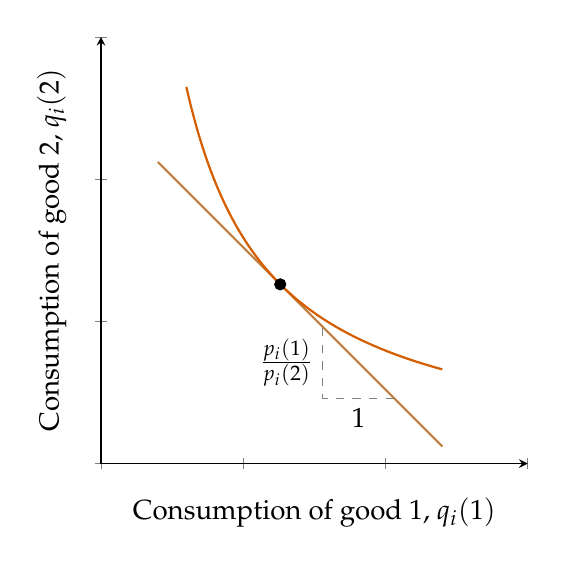
\begin{tikzpicture}
            \pgfmathsetmacro{\beta}{1/3}
            \pgfmathsetmacro{\alpha}{0.5}
        
            \pgfmathsetmacro{\Zm}{1}
            \pgfmathsetmacro{\K}{1}
            
            \pgfmathsetmacro{\Za}{1}
            \pgfmathsetmacro{\T}{1}
        
            \pgfmathsetmacro{\Kf}{1}
            \pgfmathsetmacro{\Tf}{15}
        
        
            \pgfmathsetmacro{\P}{\Za/\Zm * ((1-\alpha)/\alpha * \T / \K)^(\beta)}   
        
        
            \pgfmathsetmacro{\Pw}{\Za/\Zm * ((1-\alpha)/\alpha * ( ( \T + \Tf) / (\K+\Kf ) )^(\beta)}  
            \pgfmathsetmacro{\Qw}{(1-\alpha)/\alpha / \Pw}
        
            \pgfmathsetmacro{\L}{1}
            \pgfmathsetmacro{\Omega}{(\P *\Zm / \Za)^(1/\beta) * \K / \T}      
            \pgfmathsetmacro{\Ls}{ \Omega / (1+\Omega) * \L}    
            \pgfmathsetmacro{\Ym}{ \Zm * \K^(\beta) * \Ls^(1-\beta) }
            \pgfmathsetmacro{\Ya}{ \Za * \T^(\beta) * (1-\Ls)^(1-\beta) }
        
            \pgfmathsetmacro{\Omegaw}{(\Pw *\Zm / \Za)^(1/\beta) * \K / \T}      
            \pgfmathsetmacro{\Lsw}{ \Omegaw / (1+\Omegaw) * \L}    
            \pgfmathsetmacro{\Ymw}{ \Zm * \K^(\beta) * \Lsw^(1-\beta) }
            \pgfmathsetmacro{\Yaw}{ \Za * \T^(\beta) * (1-\Lsw)^(1-\beta) }
            \pgfmathsetmacro{\Iw}{ \Pw * \Ymw + \Yaw }
            \pgfmathsetmacro{\Qaw}{(1-\alpha) * \Iw}
            \pgfmathsetmacro{\Qmw}{(\alpha)/\Pw * \Iw}
        
        %    \pgfmathsetmacro{\ws}{ \Pm * \Zm * (1-\beta) * (\K / \Ls )^(\beta) }   
            % Compute utility level
            \pgfmathsetmacro{\U}{(\Ya^(\alpha))*(\Ym^(1 - \alpha))}
            \pgfmathsetmacro{\Uw}{(\Qaw^(\alpha))*(\Qmw^(1 - \alpha))}
            
            % Compute prefactor for indifference curve: Qc = A * Qr^(- (1 - alpha)/alpha)
            \pgfmathsetmacro{\expo}{\alpha/(1 - \alpha)}
            \pgfmathsetmacro{\A}{\U^(1/\alpha)}
            \pgfmathsetmacro{\Aw}{\Uw^(1/\alpha)}
            
            \centering
            \begin{axis}[
                xlabel={Consumption of good $1$, $q_{i}(1)$},
                ylabel={Consumption of good $2$, $q_{i}(2)$},
                ymin=0, ymax=\L+.5,
                xmin=0, xmax=\L+.5,
                yticklabel=\empty,
                xticklabel=\empty,
                axis lines=left,
                enlargelimits=false,
                clip=false,
                axis on top,
                scaled x ticks=false,
                width=7cm, height=7cm,
                title style={font=\bfseries}
            ]
            
            % PPF: Q_C = (L/a_C) - (a_R/a_C) * Q_R
            \pgfmathsetmacro{\c}{ \Ym + \P * \Ya }
            \addplot[thick, brown, domain=0.2:1.2] { \c - \P*x};
        
            \addplot[thick, red, domain=0.3:1.2, samples=100] {\A * x^(-\expo)};

            
            
            % Labels
            %\node at (axis cs:3.5,0.03) {\Large $\mathcal{Y}_{US}$};
            %\node at (axis cs:\Lendow/\aR,-.01) {\scriptsize $\frac{L_{US}}{a_{US,R}}$};
            %\node at (axis cs:-.75,\Lendow/\aC) {\scriptsize $\frac{L_{US}}{a_{US,C}}$};
            
            
            % Equilibrium point
            \addplot[only marks, mark=*, color=black, mark size=2pt] coordinates {(\Ym, \Ya)};

            %\addplot[gray, dashed] coordinates {(0,\Ym) (\Ym,\Ya) (\Ya,0)};

            \pgfmathsetmacro{\sx}{\Ym+.4}
            \pgfmathsetmacro{\sy}{\c - \P*\sx};
            \pgfmathsetmacro{\ssx}{\sx-.25};
            \pgfmathsetmacro{\ssy}{\c - \P*\ssx};
            
            %\addplot[only marks, mark=*, color=black, mark size=2pt] coordinates {(\sx,\sy)};
            \addplot[gray, dashed] coordinates {(\sx,\sy) (\ssx,\sy) (\ssx,\ssy)};
            \node[anchor=north] at (axis cs: {\ssx + (\sx-\ssx)/2},\sy) {$1$};
            \node[anchor=east] at (axis cs: {\ssx},{\ssy - (\ssy - \sy)/2}) {$\frac{p_i(1)}{p_i(2)}$};
            
           
            
            \end{axis}
            \end{tikzpicture}

        }

            \end{column}
\end{columns}
\end{frame}


\begin{frame}{Demand functions}
\begin{columns}
    \begin{column}{0.5\textwidth}
       After some algebra, we can solve for demand functions:            
        \begin{equation*}
            q_i(\varphi) = \underbrace{\left( \frac{p_i(\varphi)}{P_i} \right)^{-\sigma}}_{\text{relative price}} \times \underbrace{\frac{I_i}{P_i}}_{\text{real income}}
            \end{equation*}
        {\scriptsize \qquad \textcolor{gray}{(check handout for step by step derivation)}}

       \begin{wideitemize}
        \item<2-> \blue{Intuition}: demand is...
        \begin{itemize}
            \item ...decreasing in the relative price
            \item ...increasing in real aggregate income
        \end{itemize}        

        \item<3-> What about $\sigma$?
        \begin{itemize}
            \item<4-> $\sigma$ small: large change in price, small drop in demand
            \item<5-> $\sigma$ large: small change in price, large drop in demand
        \end{itemize}
        \end{wideitemize}


    \end{column}
    
    \begin{column}{0.5\textwidth}
    \onslide<6->{
    \begin{figure}[htp]
        \centering
        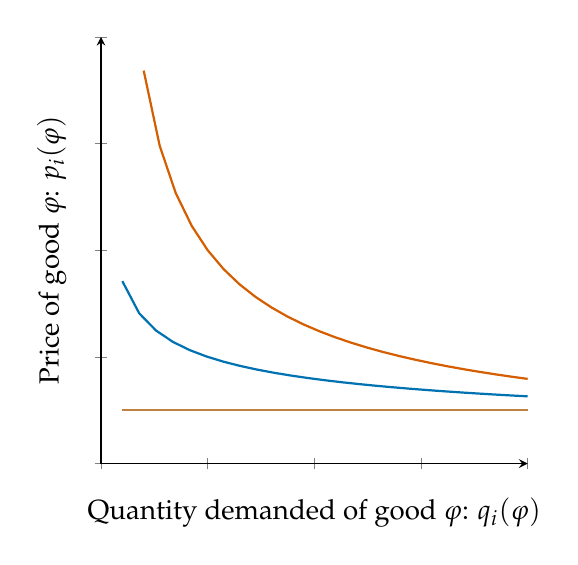
\begin{tikzpicture}
        \pgfmathsetmacro{\sigmaa}{1.5}
        \pgfmathsetmacro{\sigmab}{3}
        \pgfmathsetmacro{\sigmac}{10000000}
        \pgfmathsetmacro{\P}{0.25}
        \pgfmathsetmacro{\I}{1}
        
        \centering
        \begin{axis}[
            ylabel={Price of good $\varphi$: $p_i(\varphi)$},
            xlabel={Quantity demanded of good $\varphi$: $q_i(\varphi)$},
            ymin=0, ymax=2,
            xmin=0, xmax=2,
            yticklabel=\empty,
            xticklabel=\empty,
            axis lines=left,
            enlargelimits=false,
            clip=false,
            axis on top,
            scaled x ticks=false,
            width=7cm, height=7cm,
            title style={font=\bfseries}
        ]
        
        % PPF: Q_C = (L/a_C) - (a_R/a_C) * Q_R
    
        
          \addplot[thick,red,  domain=0.2:2]
            {\P * ((x*\P)/\I)^(-1/\sigmaa)};
          \addplot[thick,blue, domain=0.1:2]
            {\P * ((x*\P)/\I)^(-1/\sigmab)};
          \addplot[thick,brown,domain=0.1:2]
            {\P};  % σ → ∞  ⇒  horizontal line at p = P
            
        \end{axis}
    
    \end{tikzpicture}
            \caption{Demand curve with different elasticities: \textcolor{red}{$\sigma=1.5$, \textcolor{blue}{$\sigma=3$}, \textcolor{brown}{$\sigma=\infty$}}}
        \label{fig: ces-demand}
    \end{figure}
    
        }

            \end{column}
\end{columns}
\end{frame}

\section{Production}

\begin{frame}{Production}

\begin{wideitemize}
    \item Producers of each good $\varphi$ have a monopoly over the production of their good
    \item They also will have to pay a fixed cost $\bar{f}$ to set up shop (only if they enter the market)

    \item To produce a given quantity $q_i(\varphi)$, labor used is:

    \begin{equation*}
         \ell = \bar{f} + a^*q_i(\varphi) \iff q_i(\varphi) = \frac{1}{a^*} (\ell - \bar{f})
    \end{equation*}

    \item $a^*$: denotes how many workers are necessary to produce a single unit of good $\varphi$. \\
    \qquad (\blue{unit labor requirements}, as we have seen in the Ricardian model) 

    \item Only labor $\ell > \bar{f}$ contributes to extra production
    \item \blue{What does this mean for economies of scale?}
\end{wideitemize}
    
\end{frame}

\begin{frame}{Fixed costs and increasing return}
    \begin{center}
    \begin{tikzpicture}
    \pgfmathsetmacro{\m}{1}
    \pgfmathsetmacro{\f}{.250}
    \begin{axis}[
        ylabel={Output $q_i(\varphi)$},
        xlabel={Labor $\ell$},
        ymin=0, ymax=1,
        xmin=0, xmax=1,
        yticklabel=\empty,
        xticklabel=\empty,
        axis lines=left,
        enlargelimits=false,
        clip=false,
        axis on top,
        scaled x ticks=false,
        width=7cm, height=6cm,
        title style={font=\bfseries}
    ]

        \addplot[green, thick, domain=0:1] {max(0,\m * (x-\f))};

        \node[anchor = north] at (axis cs: .250, 0) {$\bar{f}$};

    \end{axis}
    \end{tikzpicture}
    \end{center}
\end{frame}

\begin{frame}{Cost functions}

\begin{itemize}
    \item \blue{Total cost} for producing output up to level $q$ is:

    \begin{equation*}
        C(q) = \underbrace{\bar{f}w_i}
        _{\text{fixed cost}} + \underbrace{a^*w_i \times q}_{\text{variable cost}}
    \end{equation*}

    \item<2-> \blue{Marginal costs} are constant (independent of level $q$):

    \begin{equation*}
        MC = C'(q) = a^* w_i
    \end{equation*}

    \item<3-> \blue{Average costs} are decreasing in $q$:

    \begin{equation*}
        AC(q) = \frac{C(q)}{q} = \frac{\bar{f}w_i}{q} + a^*w_i
    \end{equation*}    

    \item<4-> $\implies$ increasing returns to scale, potential profits, monopoly power

    \item<5-> \blue{Intuition}: $\bar{f}$: ``cost of entering the market''
    
    \item<6-> New firm must pay the same up-front cost for product design, setting up a factory, etc.
    
    \item<7-> After that, producing an extra unit only costs labor at a constant marginal cost.

    
\end{itemize}
    
\end{frame}

\begin{frame}{Average and marginal cost}

    \begin{figure}[htp]
        \centering
        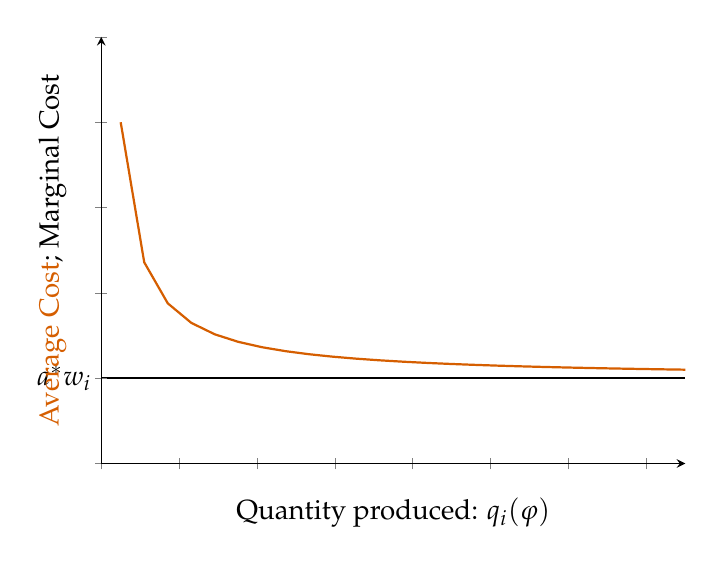
\begin{tikzpicture}

        \pgfmathsetmacro{\fbar}{1.5}
        \pgfmathsetmacro{\a}{1}
        \pgfmathsetmacro{\w}{1}
        
        \centering
        \begin{axis}[
            ylabel={\textcolor{red}{Average Cost}; Marginal Cost},
            xlabel={Quantity produced: $q_i(\varphi)$},
            ymin=0, ymax=5,
            xmin=0, xmax=15,
            yticklabel=\empty,
            xticklabel=\empty,
            axis lines=left,
            enlargelimits=false,
            clip=false,
            axis on top,
            scaled x ticks=false,
            width=9cm, height=7cm,
            title style={font=\bfseries}
        ]
        
        
          \addplot[thick,red,  domain=0.5:15]
            {\fbar/x + \a * \w};
          \addplot[thick,black,  domain=0:15]
            {\a * \w};

            \node[anchor=east] at (axis cs: 0, \a * \w) {$a^* w_i$};
            
        \end{axis}
    
    \end{tikzpicture}
            \caption{Average cost as a function of output}
        \label{fig: ac}
    \end{figure}    
\end{frame}



\begin{frame}{Monopolist's maximization problem}

\begin{wideitemize}
    \item In competitive markets, producers take prices as given 
    \item Monopolists incorporate into their problem the fact that their choice of prices changes demand
    \item They take demand functions as given and pick price to maximize profits, maximizing:

    \begin{equation*}
        \max_{p} \pi_i = (p-MC)q(p) - w_i \bar{f}
    \end{equation*}

    \blue{Solution} (using chain rule):

    \begin{equation*}
        MR = p + \frac{q(p)}{q'(p)} = MC
    \end{equation*}

\end{wideitemize}
    
\end{frame}

\begin{frame}{Monopolist's maximization problem}

    \begin{wideitemize}
            \item Recall:

    \begin{equation*}
        q(p) = \left( \frac{p}{P_i} \right)^{-\sigma} \times \frac{I_i}{P_i}, \qquad q'(p) = -\sigma \times \frac{1}{p} \times \left( \frac{p}{P_i} \right)^{-\sigma} \times \frac{I_i}{P_i}  = -\sigma \times \frac{1}{p} \times q(p)
    \end{equation*}

    \item<2-> Hence: 

    \begin{eqnarray*}
        p + \frac{q(p)}{q'(p)} &=& MC \\
        p - \frac{p}{\sigma} &=& MC \\
p^* &=& \frac{\sigma}{\sigma -1}\times MC 
    \end{eqnarray*}

    \item<3-> Note $\frac{\sigma}{\sigma -1} > 1$. We call this a mark-up. \\
    \qquad \textcolor{gray}{(what happens when $\sigma \to \infty$?)}
    \item<4-> \blue{Optimal price = mark-up $\times$ marginal cost.}

    
    \end{wideitemize}
\end{frame}


\begin{frame}{Monopolistic competition}
\centering
    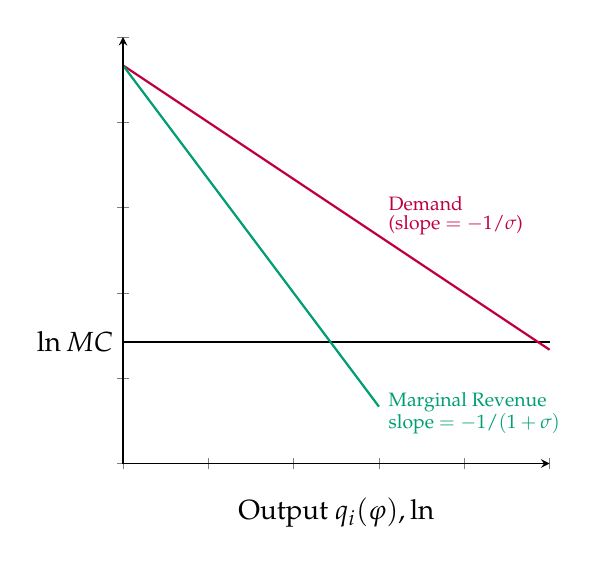
\begin{tikzpicture}
    \pgfmathsetmacro{\K}{7}
    \pgfmathsetmacro{\sigmaa}{1.5}

    \pgfmathsetmacro{\A}{7}
    \pgfmathsetmacro{\b}{0.75}
    \pgfmathsetmacro{\m}{0.35}
    \pgfmathsetmacro{\pmax}{\A/\b}          % choke price  (demand intercept)
    \pgfmathsetmacro{\qc}{\A - \b/\m}       % competitive quantity (P = MC)
        
    
    
    \begin{axis}[
        xlabel={Output $q_i(\varphi), \ln$},
        ymin=0, ymax=10,
        xmin=0, xmax=5,
        yticklabel=\empty,
        xticklabel=\empty,
        axis lines=left,
        enlargelimits=false,
        clip=false,
        axis on top,
        scaled x ticks=false,
        width=7cm, height=7cm,
        title style={font=\bfseries}
    ]

        \pgfmathsetmacro{\q}{((\A / \b - 1/ \m ) / ( 2/\b))}
        \pgfmathsetmacro{\p}{ (\A / \b) - 1/\b * \q }
        
            
        \addplot[black, thick, domain=0:5] {1/\m};
        \addplot[purple, thick, domain=0:5] {(\A / \b) - 1/\b * x};
        \addplot[green, thick, domain=0:3] {(\A / \b) - 2/\b * x};
        %\pgfmathsetmacro{\f}{\p * \q - \q / \m}
        %\addplot[blue, thick, domain=1:5] {1/\m + \f / x};


        %\addplot[gray, dashed] coordinates {(\q,1/\m + \f / \q) (0,1/\m + \f / \q)};
        %\addplot[only marks, mark=*, color=black, mark size=2pt] coordinates {(\q,1/\m + \f / \q)};

        %\node[anchor=south west] at (axis cs: 5,{1/\m+.43}) {\textcolor{blue}{Average Cost}};
        \node[anchor=west] at (axis cs: 3,\p) {\scriptsize \textcolor{purple}{Demand}};
        \node[anchor=west] at (axis cs: 3,\p-.5) {\scriptsize \textcolor{purple}{(slope $= - 1/\sigma$)}};
        \node[anchor=west] at (axis cs: 3,{1/(2*\m)}) {\textcolor{green}{\scriptsize Marginal Revenue}};
        \node[anchor=west] at (axis cs: 3,{1/(2*\m)-.5}) {\textcolor{green}{\scriptsize slope $= - 1/(1+\sigma)$}};
        \node[anchor=east] at (axis cs: 0,1/ \m) {$\ln  MC$};
    \end{axis}

    \end{tikzpicture}

 \end{frame}


\begin{frame}{Monopolistic competition}
\addtocounter{framenumber}{-1}
\centering
    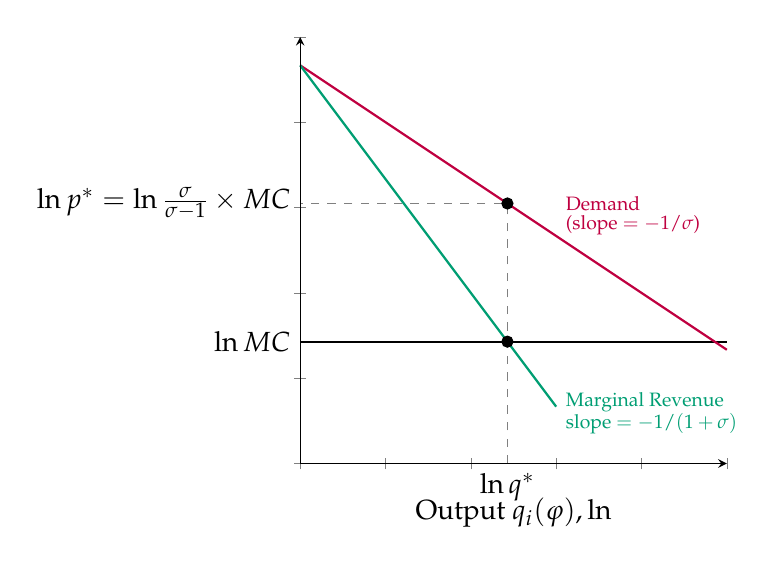
\begin{tikzpicture}
    \pgfmathsetmacro{\K}{7}
    \pgfmathsetmacro{\sigmaa}{1.5}

    \pgfmathsetmacro{\A}{7}
    \pgfmathsetmacro{\b}{0.75}
    \pgfmathsetmacro{\m}{0.35}
    \pgfmathsetmacro{\pmax}{\A/\b}          % choke price  (demand intercept)
    \pgfmathsetmacro{\qc}{\A - \b/\m}       % competitive quantity (P = MC)
        
    
    
    \begin{axis}[
        xlabel={Output $q_i(\varphi), \ln$},
        ymin=0, ymax=10,
        xmin=0, xmax=5,
        yticklabel=\empty,
        xticklabel=\empty,
        axis lines=left,
        enlargelimits=false,
        clip=false,
        axis on top,
        scaled x ticks=false,
        width=7cm, height=7cm,
        title style={font=\bfseries}
    ]

        \pgfmathsetmacro{\q}{((\A / \b - 1/ \m ) / ( 2/\b))}
        \pgfmathsetmacro{\p}{ (\A / \b) - 1/\b * \q }
        
            
        \addplot[black, thick, domain=0:5] {1/\m};
        \addplot[purple, thick, domain=0:5] {(\A / \b) - 1/\b * x};
        \addplot[green, thick, domain=0:3] {(\A / \b) - 2/\b * x};
        %\pgfmathsetmacro{\f}{\p * \q - \q / \m}
        %\addplot[blue, thick, domain=1:5] {1/\m + \f / x};

        
        \addplot[gray, dashed] coordinates {(\q,0) (\q,\p) (0,\p)};
        \addplot[only marks, mark=*, color=black, mark size=2pt] coordinates {(\q,\p)};
        \addplot[only marks, mark=*, color=black, mark size=2pt] coordinates {(\q,1/\m)};

        %\addplot[gray, dashed] coordinates {(\q,1/\m + \f / \q) (0,1/\m + \f / \q)};
        %\addplot[only marks, mark=*, color=black, mark size=2pt] coordinates {(\q,1/\m + \f / \q)};

        %\node[anchor=south west] at (axis cs: 5,{1/\m+.43}) {\textcolor{blue}{Average Cost}};
        \node[anchor=west] at (axis cs: 3,\p) {\scriptsize \textcolor{purple}{Demand}};
        \node[anchor=west] at (axis cs: 3,\p-.5) {\scriptsize \textcolor{purple}{(slope $= - 1/\sigma$)}};
        \node[anchor=west] at (axis cs: 3,{1/(2*\m)}) {\textcolor{green}{\scriptsize Marginal Revenue}};
        \node[anchor=west] at (axis cs: 3,{1/(2*\m)-.5}) {\textcolor{green}{\scriptsize slope $= - 1/(1+\sigma)$}};

        \node[anchor=east] at (axis cs: 0,\p) {$\ln p^{*}=\ln \frac{\sigma}{\sigma-1}\times MC$};
        \node[anchor=east] at (axis cs: 0,1/ \m) {$\ln  MC$};

        \node[anchor=north] at (axis cs: \q,0) {$\ln q^*$};
    \end{axis}

    \end{tikzpicture}

 \end{frame}

\begin{frame}{Monopolistic competition}
\addtocounter{framenumber}{-1}
\centering
    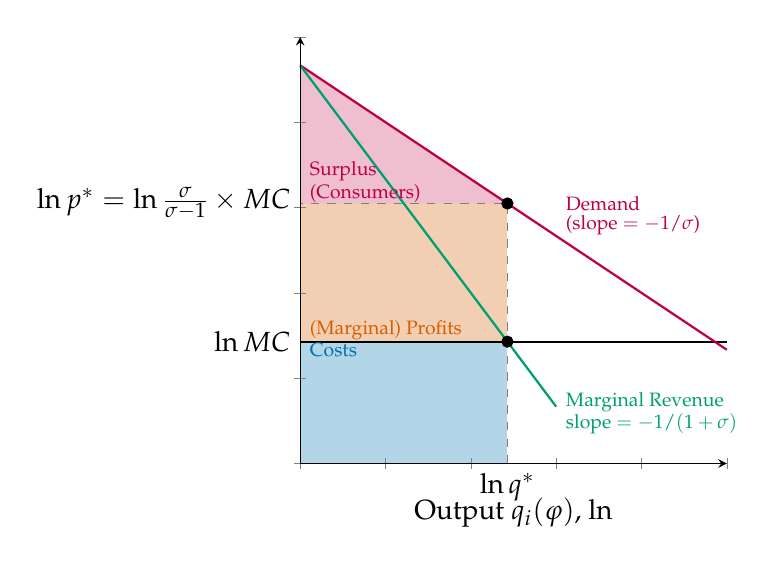
\begin{tikzpicture}
    \pgfmathsetmacro{\K}{7}
    \pgfmathsetmacro{\sigmaa}{1.5}

    \pgfmathsetmacro{\A}{7}
    \pgfmathsetmacro{\b}{0.75}
    \pgfmathsetmacro{\m}{0.35}
    \pgfmathsetmacro{\pmax}{\A/\b}          % choke price  (demand intercept)
    \pgfmathsetmacro{\qc}{\A - \b/\m}       % competitive quantity (P = MC)
        
    
    
    \begin{axis}[
        xlabel={Output $q_i(\varphi)$, ln},
        ymin=0, ymax=10,
        xmin=0, xmax=5,
        yticklabel=\empty,
        xticklabel=\empty,
        axis lines=left,
        enlargelimits=false,
        clip=false,
        axis on top,
        scaled x ticks=false,
        width=7cm, height=7cm,
        title style={font=\bfseries}
    ]

        \pgfmathsetmacro{\q}{((\A / \b - 1/ \m ) / ( 2/\b))}
        \pgfmathsetmacro{\p}{ (\A / \b) - 1/\b * \q }
        % profits
        \addplot[fill=red!30, draw=none] coordinates
            {(0,1/\m) (0,\p) (\q,\p) (\q,1/\m)} -- cycle;
        % costs
        \addplot[fill=blue!30, draw=none] coordinates
            {(0,0) (0,1/\m) (\q,1/\m) (\q,0)} -- cycle;
        % consumer-surplus
        \addplot[fill=purple!25, draw=none] coordinates
            {(0,\p) (0,\pmax) (\q,\p)} -- cycle;
        
            
        \addplot[black, thick, domain=0:5] {1/\m};
        \addplot[purple, thick, domain=0:5] {(\A / \b) - 1/\b * x};
        \addplot[green, thick, domain=0:3] {(\A / \b) - 2/\b * x};
        %\pgfmathsetmacro{\f}{\p * \q - \q / \m}
        %\addplot[blue, thick, domain=1:5] {1/\m + \f / x};

        
        \addplot[gray, dashed] coordinates {(\q,0) (\q,\p) (0,\p)};
        \addplot[only marks, mark=*, color=black, mark size=2pt] coordinates {(\q,\p)};
        \addplot[only marks, mark=*, color=black, mark size=2pt] coordinates {(\q,1/\m)};

        %\addplot[gray, dashed] coordinates {(\q,1/\m + \f / \q) (0,1/\m + \f / \q)};
        %\addplot[only marks, mark=*, color=black, mark size=2pt] coordinates {(\q,1/\m + \f / \q)};

        \node[anchor = south west] at (axis cs: 0,{\p+.3}) {\scriptsize \textcolor{purple}{Surplus}};
        \node[anchor = south west] at (axis cs: 0,{\p-.2}) {\scriptsize \textcolor{purple}{(Consumers)}};
        \node[anchor = south west] at (axis cs: 0,{1/(\m)-.2}) {\scriptsize \textcolor{red}{(Marginal) Profits}};
        \node[anchor = north west] at (axis cs: 0,{1/(\m)+.2}) {\scriptsize \textcolor{blue}{Costs}};

        %\node[anchor=south west] at (axis cs: 5,{1/\m+.43}) {\textcolor{blue}{Average Cost}};
        \node[anchor=west] at (axis cs: 3,\p) {\scriptsize \textcolor{purple}{Demand}};
        \node[anchor=west] at (axis cs: 3,\p-.5) {\scriptsize \textcolor{purple}{(slope $= - 1/\sigma$)}};
        \node[anchor=west] at (axis cs: 3,{1/(2*\m)}) {\textcolor{green}{\scriptsize Marginal Revenue}};
        \node[anchor=west] at (axis cs: 3,{1/(2*\m)-.5}) {\textcolor{green}{\scriptsize slope $= - 1/(1+\sigma)$}};

        \node[anchor=east] at (axis cs: 0,\p) {$\ln p^{*}=\ln \frac{\sigma}{\sigma-1}\times MC$};
        \node[anchor=east] at (axis cs: 0,1/ \m) {$\ln  MC$};

        \node[anchor=north] at (axis cs: \q,0) {$\ln q^*$};

    \end{axis}

    \end{tikzpicture}

 \end{frame}

\begin{frame}{Takeaways (so far)}
\begin{wideitemize}
    \item Demand for differentiated goods
    \item Elasticity of substitution ($\sigma$)
    \item For all good, optimal choice implies MRS = relative prices
    \item Production under monopolistic competition, fixed costs, and IRS = profit opportunities
    \item Monopoly power implies $p^* > MC$
    \item In our framework, prices = mark up over MC.
    \end{wideitemize}
 \end{frame}

\begin{frame}{Next class}
\begin{wideitemize}
    \item How to solve for the equilibrium of this model?
    \item What are the prices $\{p^*, P_i\}$, quantities demanded $\{q^*,Q_i\}$, goods in eqm $\{N\}$?
    \item What happens once we open up to trade?
    \end{wideitemize}
 \end{frame}



%----------------------------------------------------------------------%
%----------------------------------------------------------------------%


\end{document}
